\sloppy
\chapter{UVOD}

\sloppy
\section*{Kontrola verzija}

Zakir Šehić - opis firme, vizija i misija, polje djelovanja, analiza Narodnog pozorišta Sarajevo.

\noindent Benjamin Baždar - opseg projekta, obuhvaćeni moduli, neobuhvaćeni segmenti, dijagram modula i podmodula.

\noindent Emir Duvnjak - analiza \textit{CineStar} i Kupikartu.ba.

\noindent Zerina Ahmetović - opis metodologija izrade za implementaciju projekta, kreiranje gantograma.

\noindent Tarik Hastor - kreiranje PERT dijagrama.

\noindent Adnan Dervišević - analiza i procjena rizika.

\sloppy
\section{Osnovne informacije o firmi}

Projekt se realizira za kulturnu instituciju, na našim prostorima najčešće prepoznatu kao \textbf{Pozorište mladih}, koja je kroz modernu \textit{online} biletarnicu transformirala način prodaje karata i interakcije sa publikom. Ključne karakteristike sistema uključuju:
\begin{itemize}
  \item \textbf{\textit{Online} prodaja karata i rezervacija}:

  Korisnici mogu birati predstave, pregledavati rasporede, rezervisati i kupovati karte putem intuitivnog interfejsa.
  
  \item \textbf{Rezervacija i obračun cijena}:

  Mogućnost odabira sjedišta, primjena raznih popusta, korištenje korisničkih kartica te pregled detalja o predstavi.
  
  \item \textbf{Angažman publike}:
  
  Ugrađen forum za ocjenjivanje i diskusiju o predstavama, gdje se interaktivni medijski sadržaji (video, slike) koriste kako bi se približile aktivnosti mlađoj publici.
  
  \item \textbf{Integracija sa društvenim mrežama i moderni načini plaćanja}: 
  
  Platforma omogućava direktnu integraciju s \textit{Instagram}-om i \textit{TikTok}-om, a podržava plaćanje kreditnim karticama, \textit{Google Pay}-om i \textit{PayPal}-om.
\end{itemize}
\needspace{6\baselineskip}
\noindent\textbf{Vizija i misija:}

\indent\textit{NameSpace} teži postati lider u digitalizaciji kulturnih događaja, pružajući inovativna rješenja koja povezuju tradicionalne umjetničke vrijednosti s modernim tehnologijama. Naša misija je povećati angažman publike, unaprijediti iskustvo posjetilaca i omogućiti transparentnost i efikasnost u organizaciji događaja. 

\noindent\textbf{Ciljana grupa:}

Sistem je osmišljen za dinamičnu i radoznalu mladu publiku koja uživa u pozorišnim doživljajima. Namijenjen je generaciji koja cijeni kreativnost, interaktivnost i jednostavan pristup svijetu pozorišta, omogućavajući im da brzo i lako istraže repertoar, odaberu najbolja mjesta i iskoriste posebne pogodnosti prilagođene njihovim potrebama.

\noindent\textbf{Polje djelovanja:}
\vspace{-0.5em}
\begin{itemize}
  \item \textbf{Regionalno tržište}:
  Primarno se fokusira na Bosnu i Hercegovinu, ali s mogućnošću širenja na cijeli Balkan.
  \item \textbf{Evropska saradnja}:
  Aktivno uspostavljanje partnerstava s evropskim kulturnim institucijama i organizacijama.
  \item \textbf{Dodatne usluge}:
  Pored prodaje karata, \textit{NameSpace} nudi marketinške i analitičke alate, te savjetodavne usluge za organizatore događaja, čime doprinosi digitalnoj transformaciji kulturnog sektora.
\end{itemize}

\newpage

\noindent\textbf{Analiza preklapanja funkcionalnosti za Narodno pozorište u Sarajevu:}
\begin{figure}[H]
    \centering
    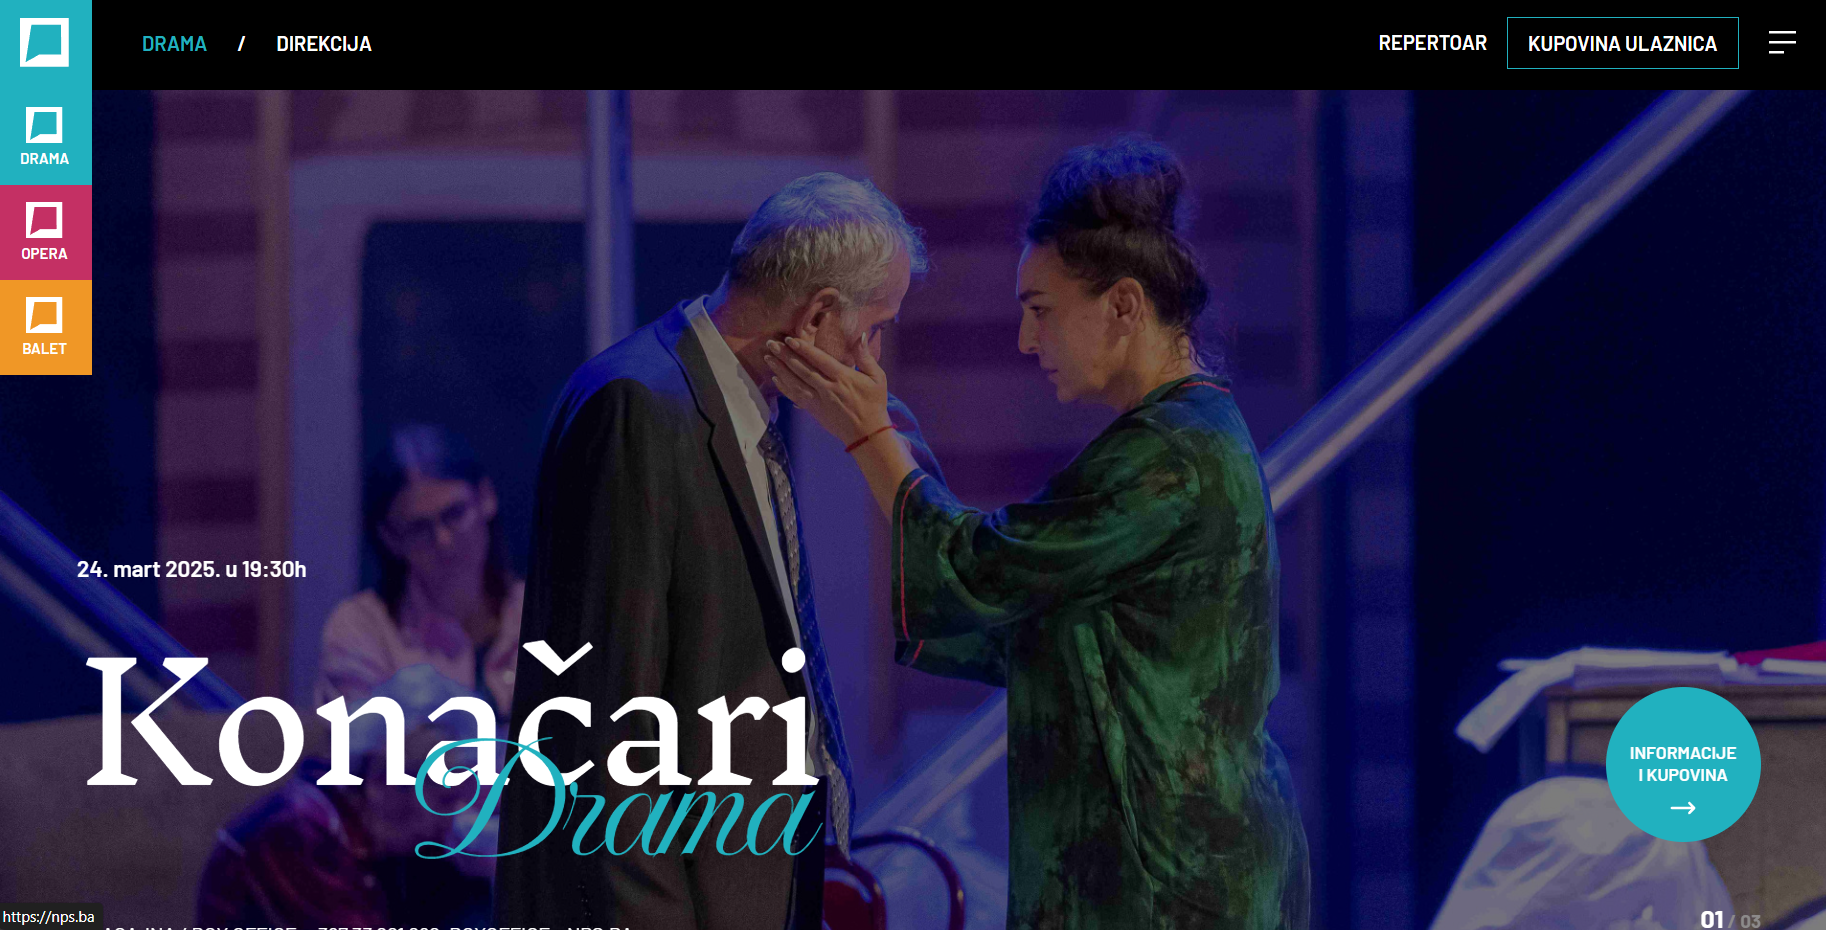
\includegraphics[width=0.8\textwidth]{Slike/narodnoPozoriste1.png}
    \caption{Naslovna stranica Narodnog pozorišta Sarajevo}
    \label{fig:np1}
\end{figure}

\begin{figure}[htbp]
    \centering
    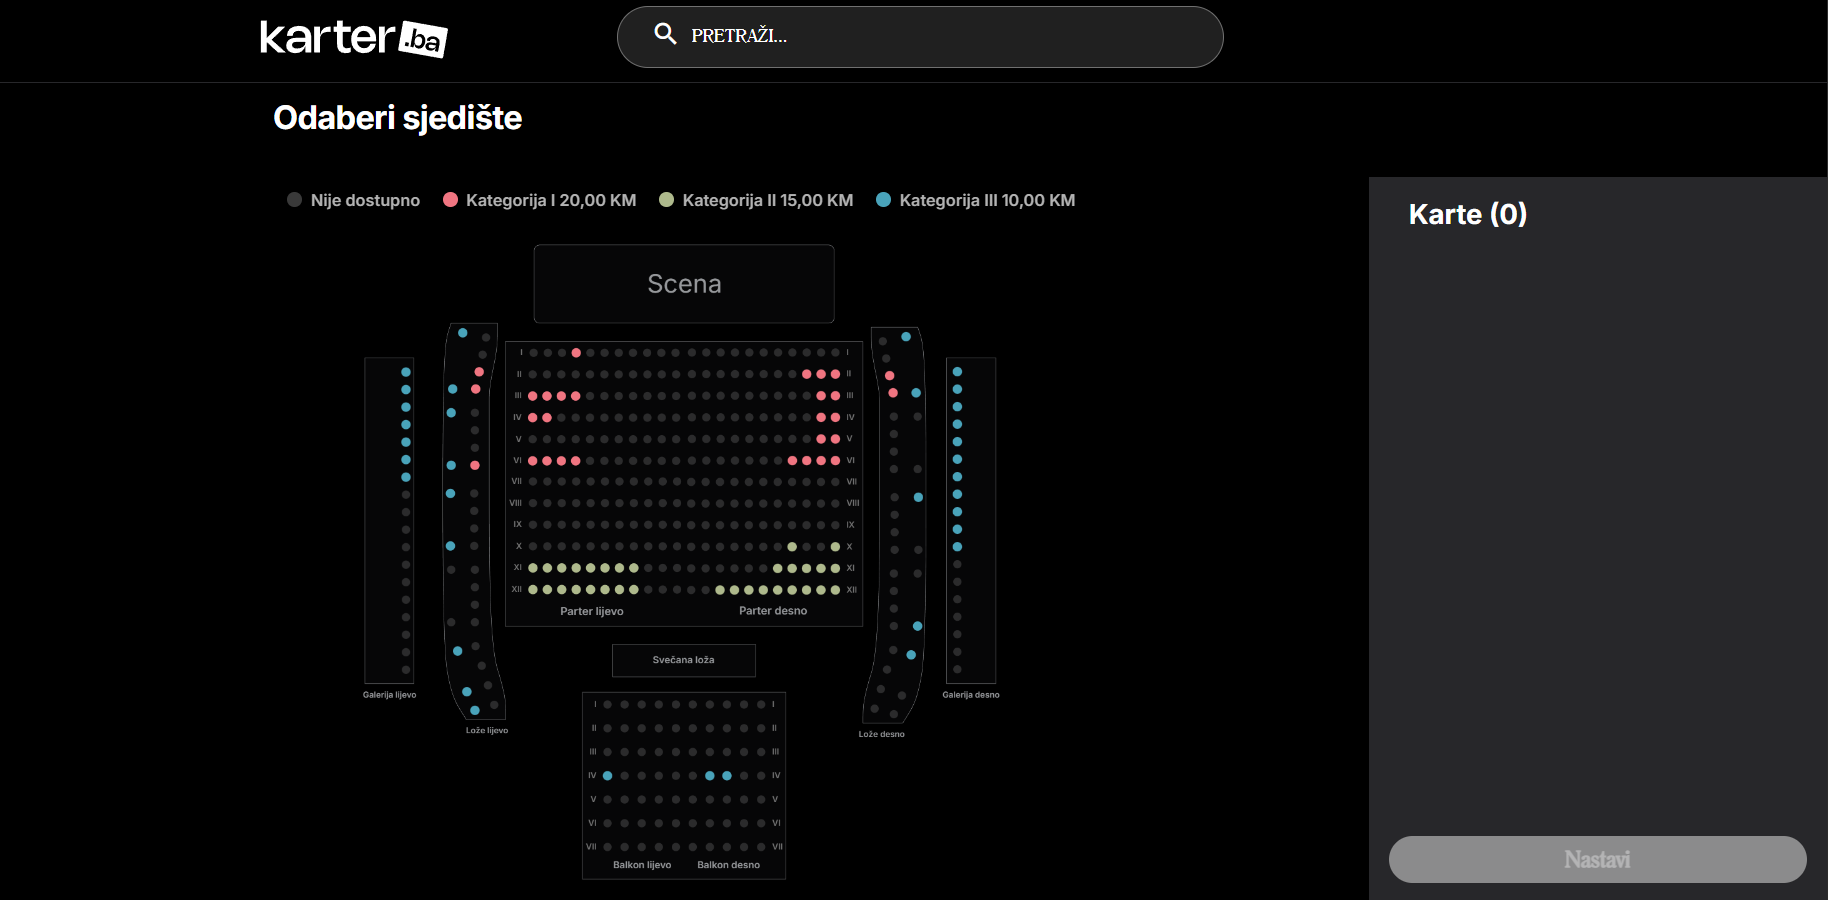
\includegraphics[width=0.8\textwidth]{Slike/narodnoPozoriste2.png}
    \caption{Rezervacija sjedišta i karte za predstavu}
    \label{fig:np2}
\end{figure}
\needspace{6\baselineskip}
Preklapanje osnovnih funkcionalnosti što uključuje \textit{online} prodaju karata, rezervaciju, pregled rasporeda i u određenoj mjeri odabir sjedišta, kako je prikazano na slici \ref{fig:np2}, je vrlo značajno između opisanog sistema i postojećeg sistema Narodnog pozorišta u Sarajevu. Međutim, napredne funkcionalnosti poput interaktivnog foruma, integracije s modernim društvenim mrežama i dodatnih metoda plaćanja predstavljaju potencijalna područja za modernizaciju i proširenje funkcionalnosti. Implementacijom ovih dodataka, naš sistem se značajno odvojio od sistema Narodnog pozorišta čime smo se bolje prilagodili zahtjevima mlađe publike i savremenim trendovima u digitalnoj komunikaciji i transakcijama.
\sloppy 

\newpage

\noindent\textbf{Analiza preklapanja funkcionalnosti za \textit{CineStar}:}
\begin{figure}[!htb]
    \centering
    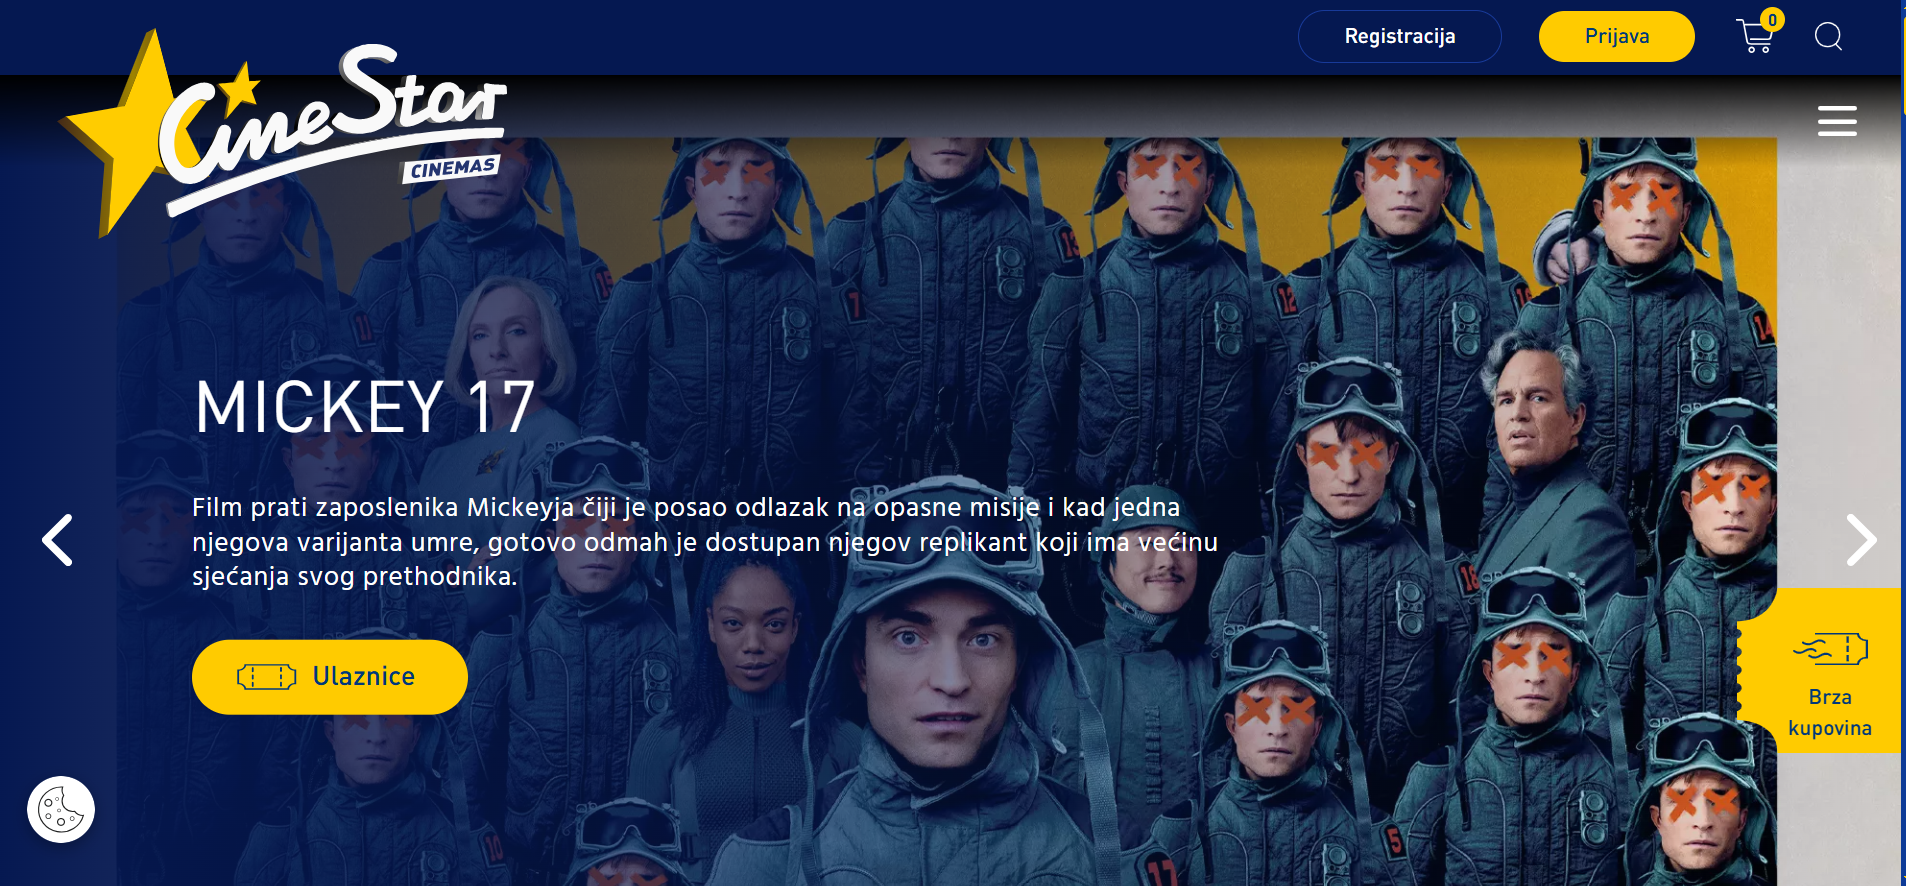
\includegraphics[width=0.8\textwidth]{Slike/cinestar1.png}
    \caption{Naslovna stranica \textit{CineStar} kina}
    \label{fig:cs1}
\end{figure}

\begin{figure}[!htb]
    \centering
    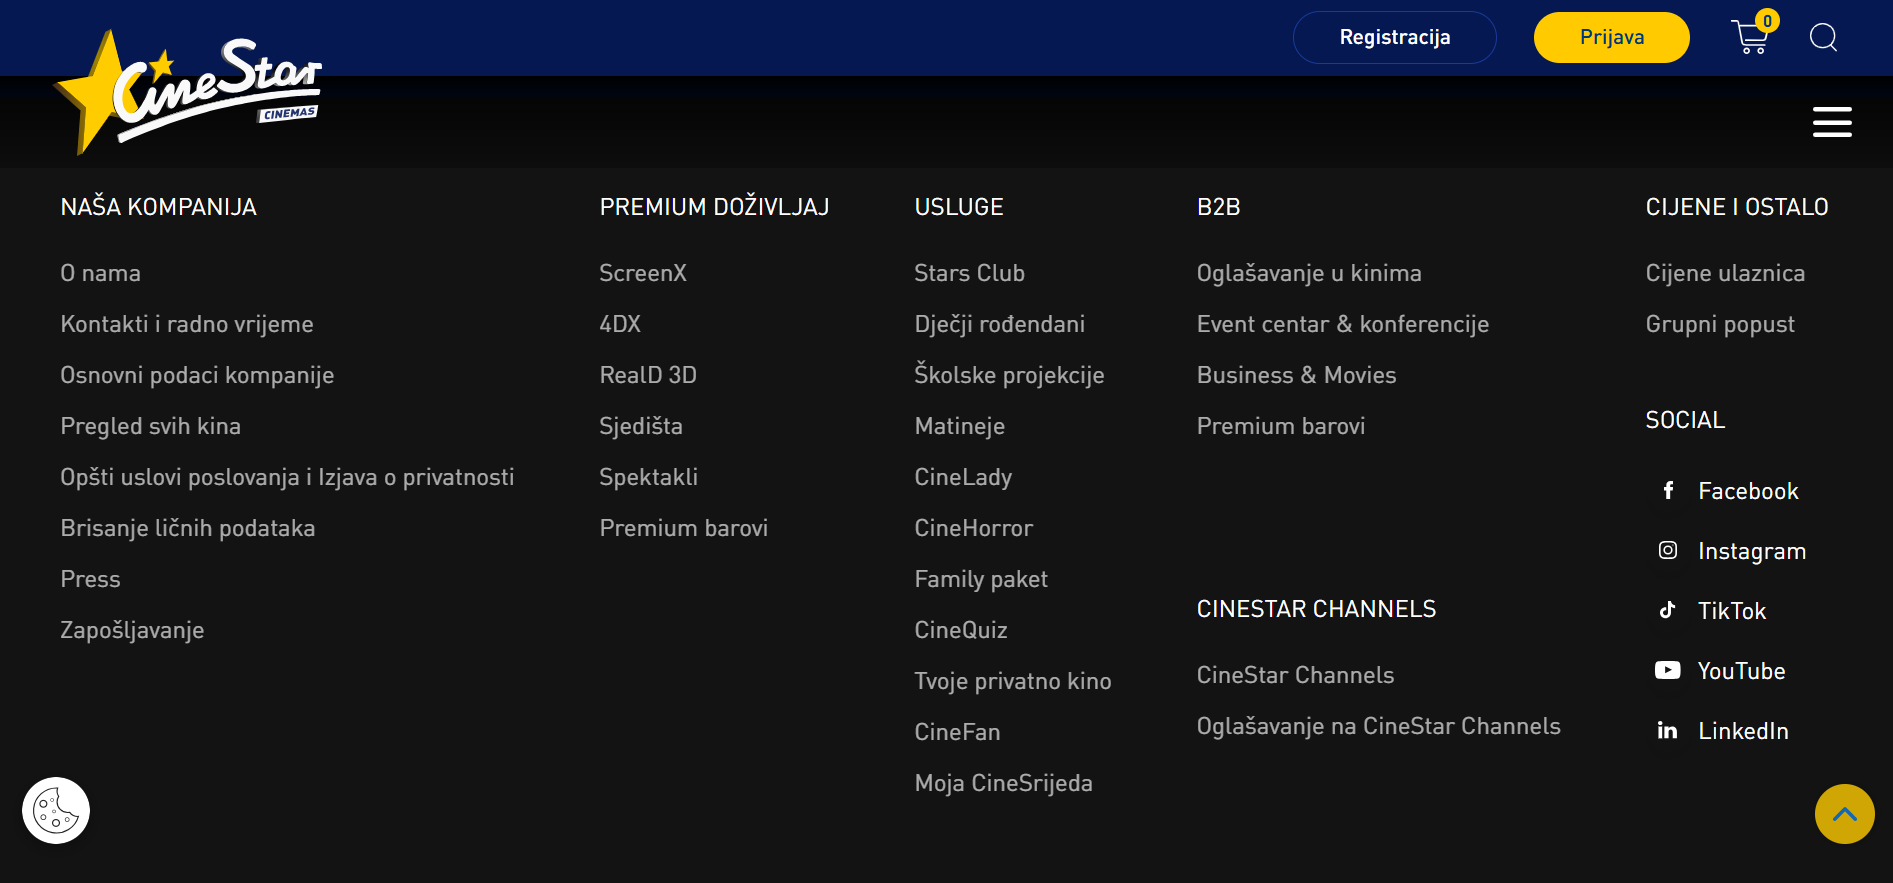
\includegraphics[width=0.8\textwidth]{Slike/cinestar2.png}
    \caption{Funkcionalnosti \textit{CineStar} sistema}
    \label{fig:cs2}
\end{figure}
\needspace{6\baselineskip}
Preklapanje funkcionalnosti između našeg sistema i \textit{CineStar}-ovog uključuje \textit{online} prodaju karata, popuste, rezervaciju, pregled rasporeda, odabir sjedišta, marketinško oglašavanje i povezanost društvenih mreža kako je prikazano na slici \ref{fig:cs2}, što je zaista većina funkcionalnosti. Međutim, implementacijom naprednih funkcionalnosti poput interaktivnog foruma i komentara korisnika kao i dodatnih metoda plaćanja, naš sistem se značajno odvojio od sistema \textit{CineStar}-a čime smo se bolje prilagodili zahtjevima mlađe publike i savremenim trendovima u digitalnoj komunikaciji i transakcijama. Naš sistem implementacijom novih društvenih mreža i foruma sa utiscima korisnika osigurava veliku transparentnost u našem poslovanju čime privlačimo mlađe korisnike čak i u doba kada kina imaju dominaciju nad pozorištima.
\sloppy 

\newpage

\noindent\textbf{Analiza preklapanja funkcionalnosti za Kupikartu.ba:}
\begin{figure}[!htbp]
    \centering
    
\includegraphics[width=0.8\textwidth]{Slike/kupikartu1.png}
    \caption{Naslovna stranica Kupikartu.ba}
    \label{fig:kk1}
\end{figure}

\needspace{6\baselineskip}
Preklapanje funkcionalnosti između našeg sistema i sistema Kupikartu.ba ogleda se prvenstveno u mogućnosti \textit{online} prodaje karata, rezervacije, pregleda rasporeda, odabira sjedišta i marketinškog oglašavanja, kao što je prikazano na slikama \ref{fig:kk2} i \ref{fig:kk3}. Ove funkcionalnosti čine značajan dio ponude oba sistema. Međutim, Kupikartu.ba je univerzalna platforma za prodaju karata za različite vrste događaja, uključujući koncerte, festivale, sportske događaje i predstave, dok je naš sistem specijalizovan isključivo za pozorište mladih. Ova usmjerenost nam omogućava da ponudimo prilagođena rješenja koja poboljšavaju iskustvo korisnika i organizatora pozorišnih događaja. Dodatno, naš sistem nudi transparentnu i interaktivnu funkcionalnost komentarisanja, omogućavajući korisnicima da ocjenjuju predstave, dijele mišljenja i daju povratne informacije. Ova opcija ne samo da podstiče angažman publike, već nam omogućava i kontinuirano unapređenje sistema na osnovu stvarnih potreba korisnika, čime se dodatno ističemo u odnosu na konkurenciju.
\sloppy 
\begin{figure}[!htb]
    \centering
    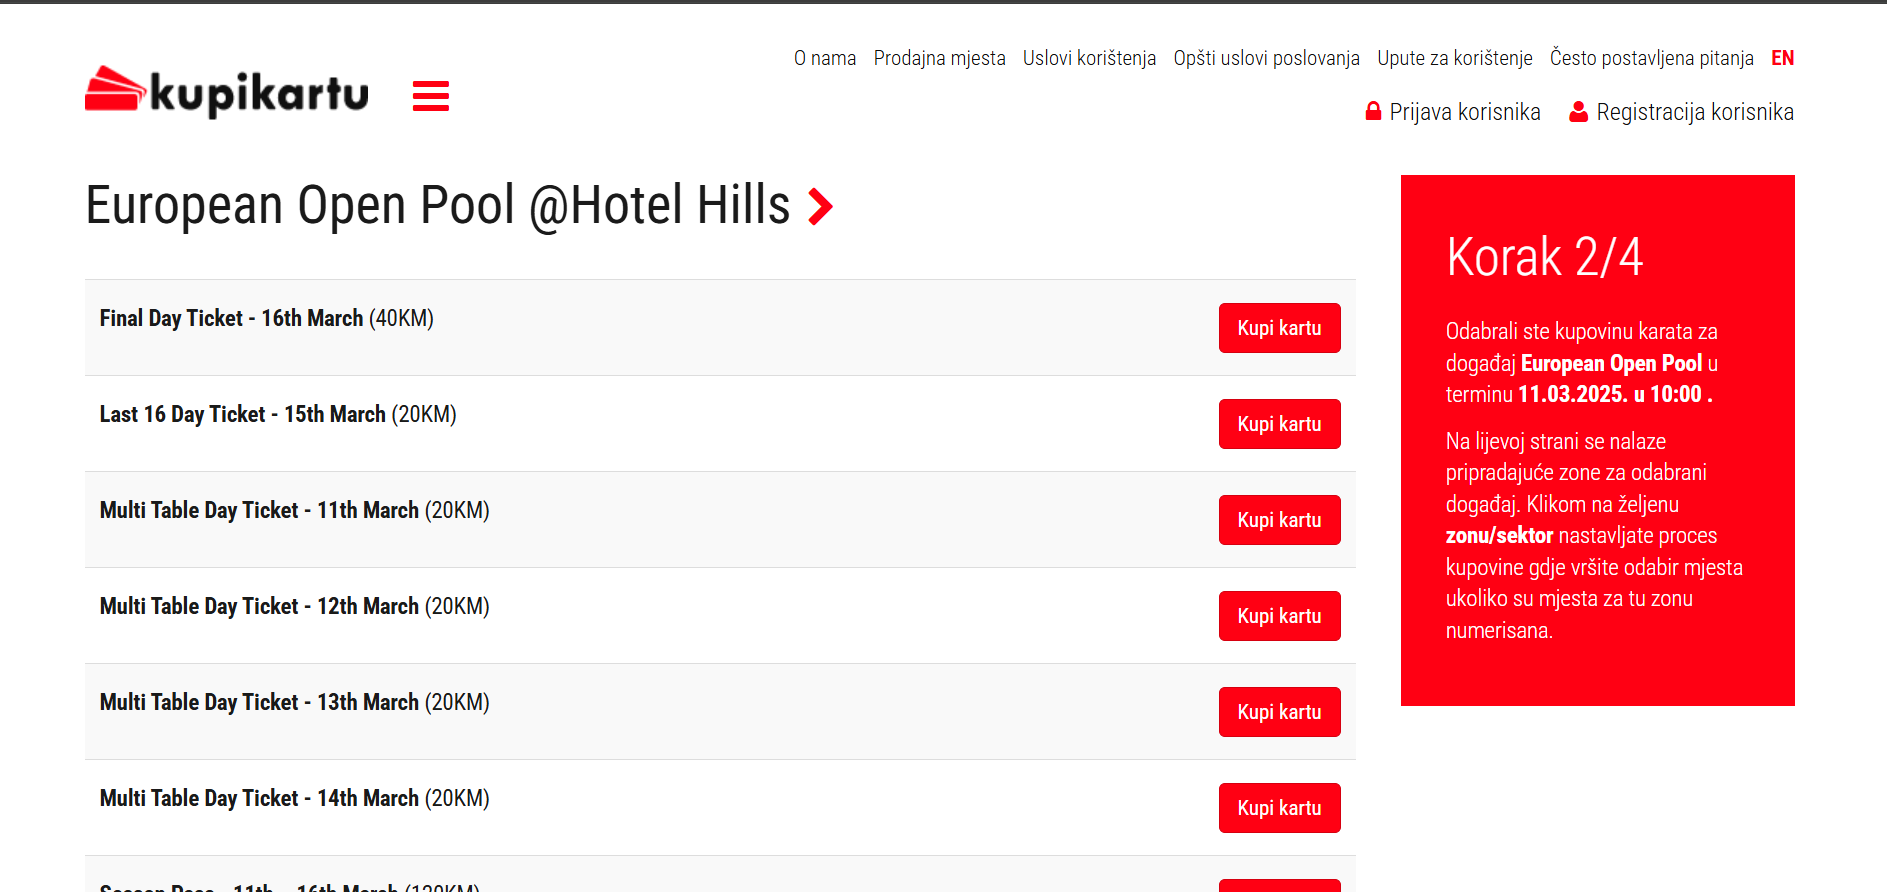
\includegraphics[width=0.8\textwidth]{Slike/kupikartu2.png}
    \caption{Kupovina karte kroz Kupikartu.ba sistem}
    \label{fig:kk2}
\end{figure}
\begin{figure}[!htb]
    \centering
    
\includegraphics[width=0.8\textwidth]{Slike/kupikartu3.png}
    \caption{Funkcionalnosti i načini plaćanja Kupikartu.ba sistema}
    \label{fig:kk3}
\end{figure}

\section{Opseg projekta}

Informacioni sistem koji se razvija za Pozorište mladih ima za cilj unapređenje digitalnog poslovanja i interakcije s publikom putem modernih tehnologija. Sistem obuhvata ključne aspekte poslovanja, ali ne uključuje određene operativne i administrativne procese koji nisu direktno povezani s prodajom i organizacijom događaja.

\subsection{Obuhvaćeni moduli}

\begin{itemize}
\item \textbf{Upravljanje repertoarom} - Unos, ažuriranje i pregled predstava, uključujući rasporede i opis sadržaja.
\item \textbf{\textit{Online} prodaja i rezervacija karata} - Mogućnost kupovine i rezervacije ulaznica putem \textit{web} platforme.
\item \textbf{Korisnički profili i lojalnost programi} - Registracija korisnika, praćenje kupovina i dodjela pogodnosti.
\item \textbf{Interaktivna komunikacija} - Forum za diskusije, ocjene i komentare posjetilaca.
\item \textbf{Marketing i promocija} - Integracija sa društvenim mrežama i slanje promotivnih obavijesti.
\item \textbf{Plaćanja i fakturisanje} - Implementacija različitih metoda plaćanja, uključujući \textit{online} transakcije.
\item \textbf{Analitika i izvještavanje} - Prikupljanje podataka o prodaji i interesovanjima korisnika radi optimizacije poslovanja.
\end{itemize}

\subsection{Neobuhvaćeni segmenti}

\begin{itemize}
\item Interno finansijsko upravljanje i knjigovodstvo.
\item Administracija zaposlenih i upravljanje resursima.
\item Tehničko održavanje objekata i infrastrukture.
\end{itemize}

Sistem je strukturisan u module i podmodule radi lakše organizacije i skalabilnosti. Na sljedećoj slici prikazan je apstraktni dijagram modula i podmodula sistema, označavajući one koji su obuhvaćeni razvojem informacionog sistema.

\begin{figure}[htbp!]
\centering
\begin{tikzpicture}[node distance=1.5cm, every node/.style={draw, align=center, minimum width=3cm}]
\node (system) {Informacioni sistem};

    \node (mod1) [below left=of system] {Upravljanje repertoarom};
    \node (mod2) [below=of system] {\textit{Online} prodaja i rezervacija};
    \node (mod3) [below right=of system] {Korisnički profili i lojalnost};
    \node (mod4) [below=of mod1] {Interaktivna komunikacija};
    \node (mod5) [below=of mod2] {Marketing i promocija};
    \node (mod6) [below=of mod3] {Plaćanja i fakturisanje};
    \node (mod7) [below=of mod5] {Analitika i izvještavanje};
    
    \draw [->] (system) -- (mod1);
    \draw [->] (system) -- (mod2);
    \draw [->] (system) -- (mod3);
    \draw [->] (mod1) -- (mod4);
    \draw [->] (mod2) -- (mod5);
    \draw [->] (mod3) -- (mod6);
    \draw [->] (mod5) -- (mod7);
\end{tikzpicture}
\caption{Dijagram modula i podmodula informacionog sistema}
\end{figure}

\section{Metodologije izrade}

Metodologije izrade koje se smatraju najpogodnijim za implementaciju informacionog sistema Pozorište mladih su navedene ispod.

\begin{enumerate}
    \item \textbf{Metodologija:} \textit{Waterfall} 

    
    \textbf{Elementi koji će se primijeniti:} Fazni razvoj, detaljna dokumentacija, sekvencijalni tok rada 

    
    \textbf{Razlozi:} Minimizira rizik od grešaka u funkcionalnostima koje ne bi smjele često mijenjati svoju strukturu ili način rada. Naročito je pogodna za module koji zahtijevaju stabilnost, preciznu dokumentaciju, konzistentnost i integritet podataka, minimalne promjene, te su u skladu sa propisima i standardima (ovakvi sistemi su upravo baze podataka, sistemi za finansijske transakcije i analitiku, tj. uključuju module Plaćanje i fakturisanje, Analitika i izvještavanje).

    \item \textbf{Metodologija:} \textit{Feature-Driven Development (FDD)} 

    
    \textbf{Elementi koji će se primijeniti:} Razvoj zasnovan na funkcionalnostima, iterativna isporuka, modeliranje objekata domene

    
    \textbf{Razlozi:} Lista funkcionalnosti je jasno definisana i neće se širiti, fokus je na postepenoj izradi pojedinačnih funkcionalnosti, odnosno modularni pristup. Omogućava se brža implementacija i testiranje funkcionalnosti, bez rizika od preklapanja ili odstupanja od specifikacija (moduli nad kojim se primjenjuje ova metodologija su \textit{Online} prodaja i rezervacija, Korisnički profili i lojalnost programi, Marketing i promocija).

    \item \textbf{Metodologija:} SCRUM 

    
    \textbf{Elementi koji će se primijeniti:} Rad u sprintovima, dnevni sastanci, povratne informacije korisnika 

    
    \textbf{Razlozi:} Fleksibilnost u razvoju korisničkog interfejsa i interaktivnih elemenata, gdje su promjene česte i poželjne. Postizanje optimalnog korisničkog iskustva, a za isto je potrebno redovno testiranje i prilagođavanje implementacije i dizajna na osnovu povratnih informacija korisnika (primjenu nalazi u implementaciji \textit{Web} interfejs-a i mobilne aplikacije, UX optimizaciji, prilagođavanju vizuelnog dizajna, te modulu Interaktivna komunikacija koji uključuje forum, ocjenjivanje, komentare).

    \item \textbf{Metodologija:} Kanban 

    
    \textbf{Elementi koji će se primijeniti:} Vizuelni prikaz toka rada, ograničenje broja aktivnih zadataka, kontinuirani razvoj i isporuka, 

    
    \textbf{Razlozi:} Omogućava kontinuirano održavanje sistema i brzo rješavanje tehničkih problema. Pomaže u organizaciji zadataka vodeći računa o prioritetima, i tako doprinosi efikasnosti tima. Smanjuje vrijeme potrebno za ispravljanje grešaka i implementaciju manjih poboljšanja i tako doprinosi stabilnosti sistema (pogodno za ažuriranje repertoara, tehničku podršku, optimizaciju sistema i sigurnost).
\end{enumerate}
Dakle, kombinacija metodologija \textit{Waterfall}, \textit{Feature-Driven Development}, SCRUM i Kanban omogućava optimalan razvoj informacionog sistema za Pozorište mladih. Ovakav pristup kombinuje strukturu i stabilnost sa agilnosti i efikasnosti, te tako osigurava visokokvalitetan razvoj i dugoročnu održivost ovog sistema.

\sloppy

\section{Plan izvedbe}
\label{izvedba}
Na slici \ref{fig:pi1} je prikaz gantograma koji vrši predikciju i raspodjelu zadataka vezanih za dokumentaciju projekta informacionog sistema. U koloni sa lijeve strane su navedene predviđene aktivnosti, kao i zadaci koje ona zahtijevaju, dok je sa desne strane vizuelni prikaz istih i predviđeno vrijeme potrebno za njihovo izvršenje.

\begin{figure}[H]
    \centering
    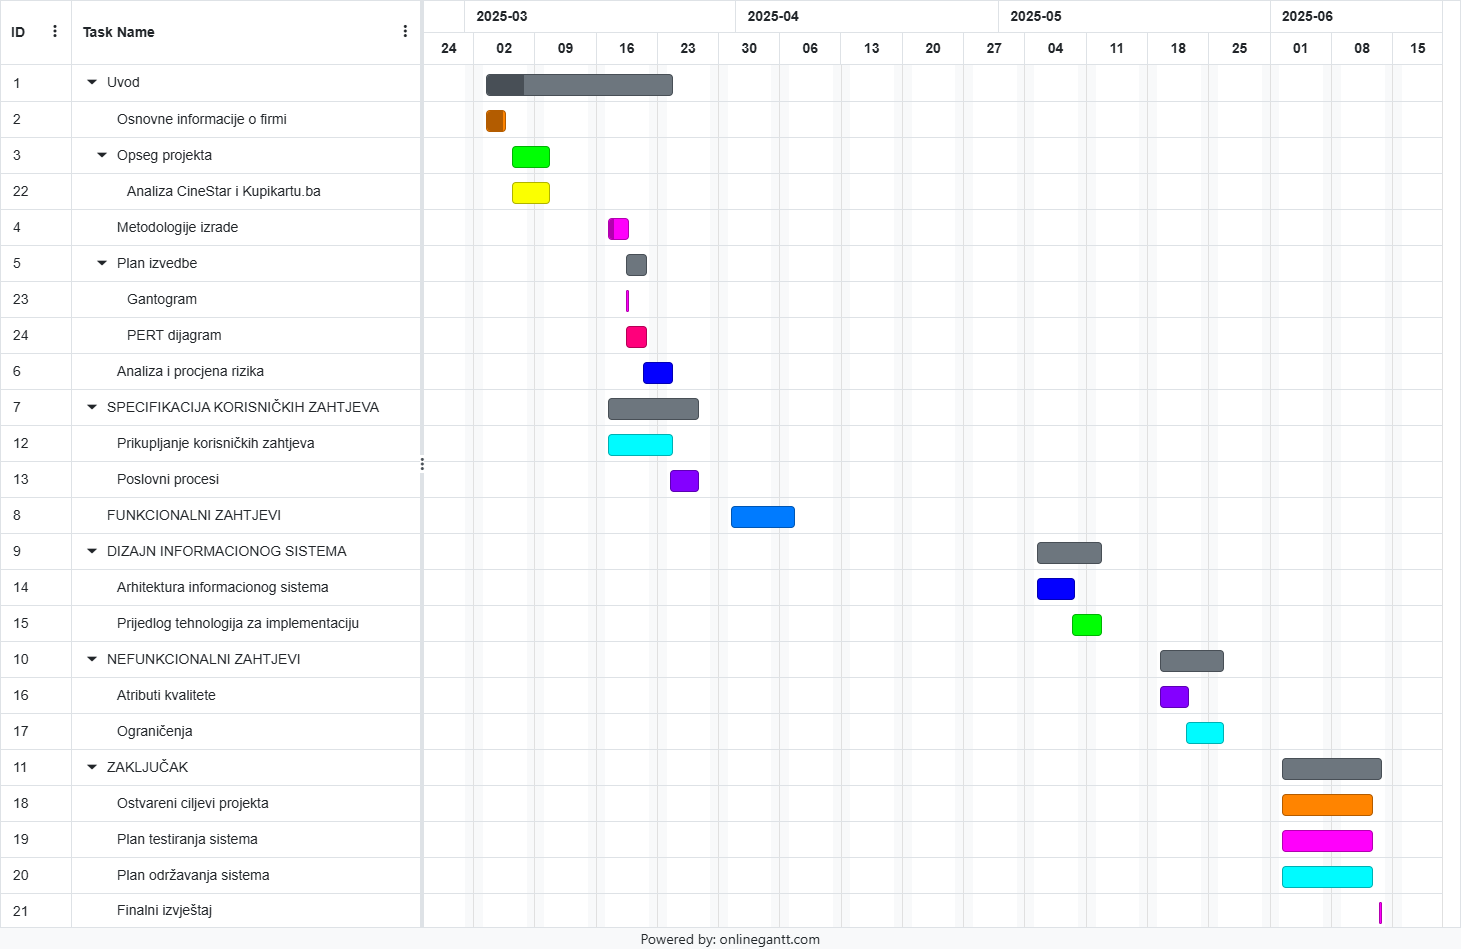
\includegraphics[width=0.8\textwidth]{Slike/gantogram.png}
    \caption{Prikaz Gantovog dijagrama sa predviđenim zadacima}
    \label{fig:pi1}
\end{figure}

Na slici \ref{fig:pi2} je vidljiv detaljniji opis Gantovog dijagrama, sa navedenim početkom, krajem i trajanjem aktivnosti, te prikazom rasporeda resursa (osoba) po zadacima, gdje je svakoj osobi dodijeljena različita boja radi lakšeg praćenja. Općenitijim aktivnostima, odnosno aktivnostima koje u sebi podrazumijevaju angažman većeg broja osoba nije dodijeljena nijedna boja (ovakve aktivnosti u sebi sadrže veći broj manjih zadataka te su po \textit{defaultu} sive boje). 

\begin{figure}[H]
    \centering
    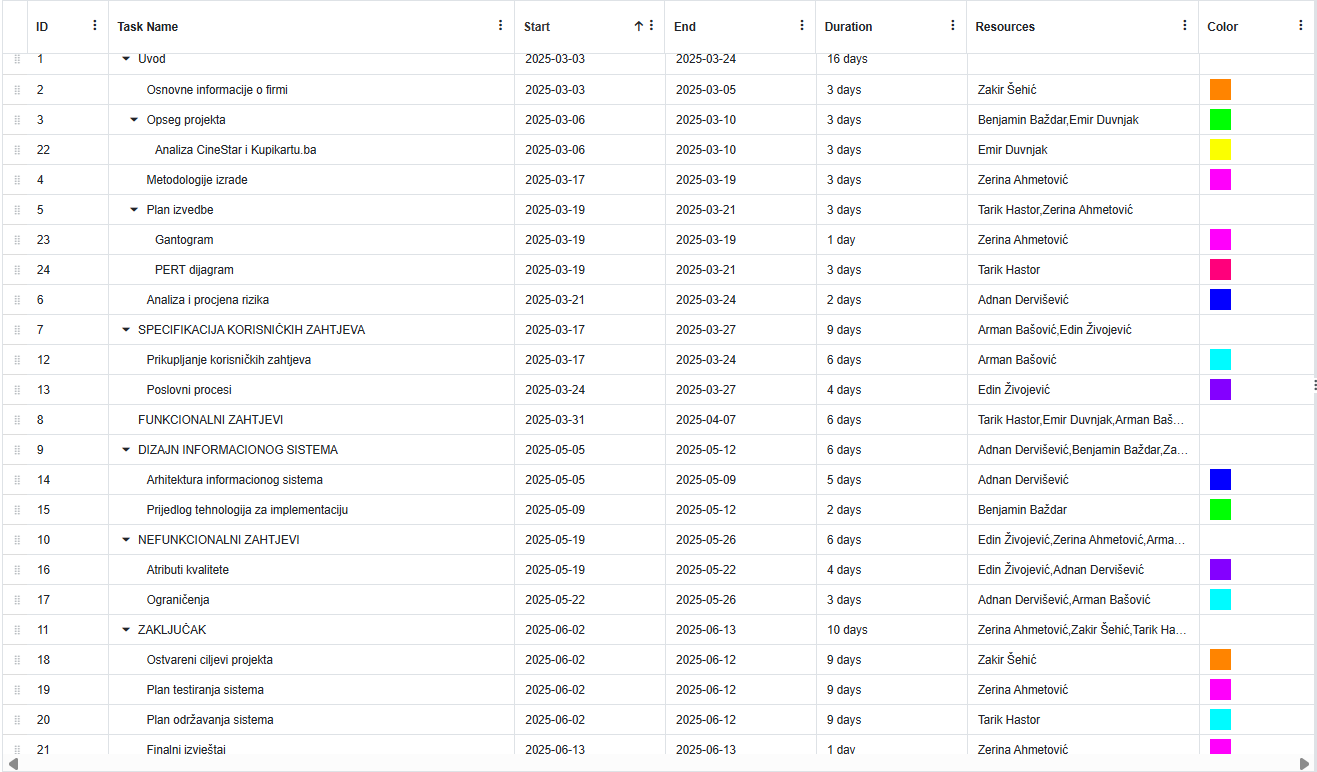
\includegraphics[width=0.8\textwidth]{Slike/gant-opis.png}
    \caption{Raspored resursa (osoba) po zadacima gantograma}
    \label{fig:pi2}
\end{figure}


Prikazano na slici \ref{fig:pi3} je "PERT" dijagram izvedbe projekta u skladu sa odabranim metodologijama. Kombinirane metodologije su:
\begin{itemize}
    \item Waterfall
    \item Feature Driven Delopment
    \item SCRUM
    \item Kanban
\end{itemize}
\begin{figure}[H]
    \centering
    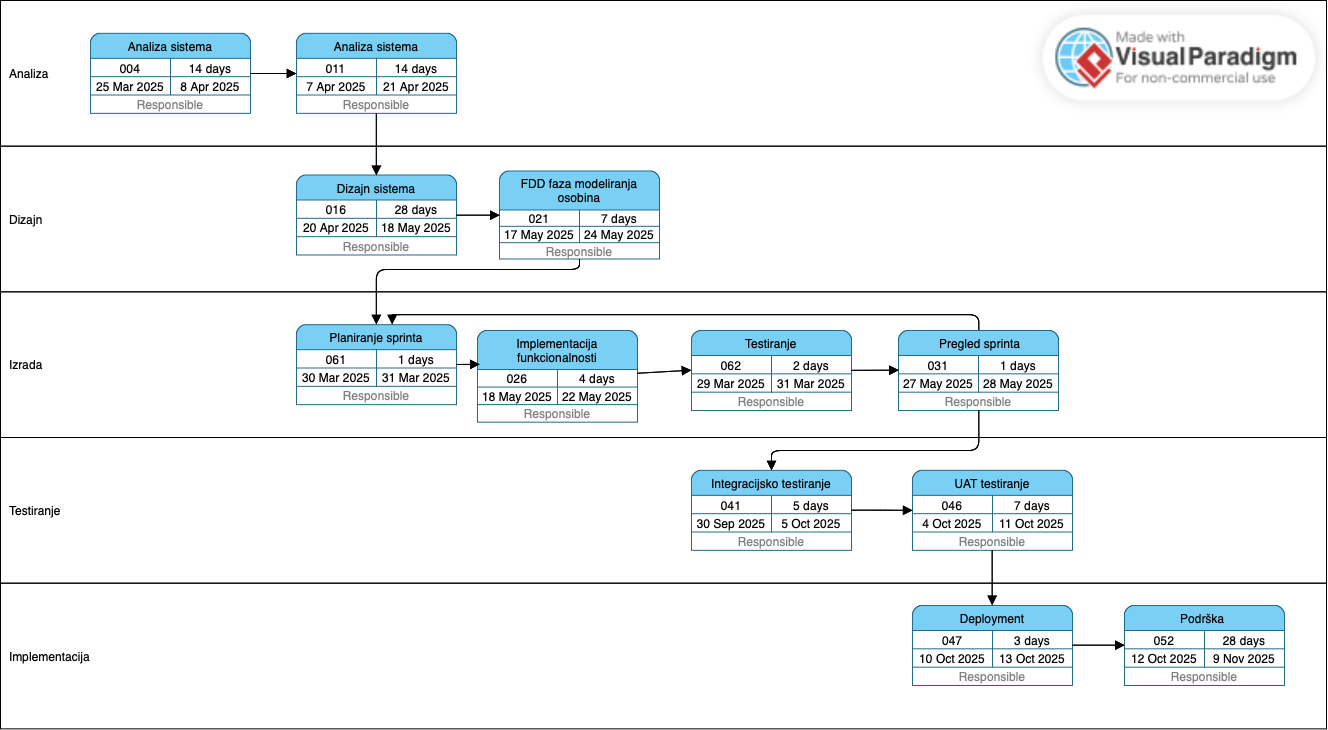
\includegraphics[width=0.8\textwidth]{Slike/PERT.png}
    \caption{Prikaz PERT dijagrama za izvedbu projekta od projektovanja do implementacije slijedeći agilne metodologije za implementaciju i waterfall za samo projektovanje.}
    \label{fig:pi3} 
\end{figure}
\newpage
\sloppy
\label{anaproc}
\section{Analiza i procjena rizika}

\begin{enumerate}
    \item \textbf{Faza rada:} Prikupljanje korisničkih zahtjeva 

    
    \textbf{Opis rizika:} U ovoj fazi postoji vremenski rizik. Ukoliko dođe do nerazumijevanja između klijenta i osoba koje prikupljaju korisničke zahtjeve, bit će potrebno odvojiti više vremena da se korisnički zahtjevi uspješno prikupe. 

    
    \textbf{Vjerovatnoća pojave:} Srednja

    \item \textbf{Faza rada:} Poslovni procesi 

    
    \textbf{Opis rizika:} U ovoj fazi postoji operativni rizik, ukoliko dođe do nerazumijevanja i manjka saradnje između osoba koje prikupljaju korisničke zahtjeve i osoba koje definišu poslovne procese. 

    
    \textbf{Vjerovatnoća pojave:} Mala

    \item \textbf{Faza rada:} Dizajn korisničkih interfejsa 

    
    \textbf{Opis rizika:} U ovoj fazi postoji finansijski rizik, jer nisu predviđena sredstva za specijalne alate za dizajniranje prototipa korisničkih interfejsa. 

    
    \textbf{Vjerovatnoća pojave:} Mala

    \item \textbf{Faza rada:} Dizajn korisničkih interfejsa 

    
    \textbf{Opis rizika:} U ovoj fazi postoji operativni rizik, zbog manjka ljudi stručnih u dizajniranju korisničkih interfejsa i njihove nepravilne raspodjele. 

    
    \textbf{Vjerovatnoća pojave:} Srednja

    \item \textbf{Faza rada:} Arhitektura informacionog sistema 

    
    \textbf{Opis rizika:} U ovoj fazi postoji tehnički rizik, zbog visoke kompleksnosti planiranja. 

    
    \textbf{Vjerovatnoća pojave:} Srednja

    \item \textbf{Faza rada:} Prijedlog tehnologija za implementaciju 

    
    \textbf{Opis rizika:} U ovoj fazi postoji vremenski rizik, jer je moguće da će biti potrebno više vremena za analizu tehnologija nego što je planirano. 

    
    \textbf{Vjerovatnoća pojave:} Mala

    \newpage
    
    \item \textbf{Faza rada:} Ograničenja 

    
    \textbf{Opis rizika:} U ovoj fazi postoji programski rizik, jer se može desiti da se nakon završetka faze pojave nova ograničenja. 

    
    \textbf{Vjerovatnoća pojave:} Mala
\end{enumerate}

